\documentclass[aspectratio=169]{beamer}

\usepackage{amsmath, amssymb}
\usepackage{bm}
\usepackage{graphicx}
\usepackage{tikz}
\usepackage{booktabs}
\graphicspath{{../../figure/}}

\usepackage{appendixnumberbeamer}


\usetheme[
        %titleformat = allsmallcaps,
        numbering = fraction, 
        progressbar = head, 
        block = fill 
        %background = dark
        ]{metropolis}
\usecolortheme{spruce}
\usefonttheme[onlymath]{serif}

\title{\Large Coexistence on the Boundary of Communities}
\subtitle{\small Dispersal in Continuum Could Lead to the Coexistence of Unstable Species Combination}
%\date{\today}
\date{\today}
\author{Chang, Longxiao, longxiao.chang@campus.lmu.de\\
Supervisor: Dr. Maria Stockenreiter}
\institute{EES, Ludwig-Maximilian Universit\"{a}t M\"{u}nchen}

\begin{document}

    \maketitle

    \begin{frame}[noframenumbering]
        \frametitle{Outline}
        \tableofcontents
    \end{frame}

    \section{Introduction}

    \begin{frame}
        Understanding biodiversity is one of the central goals of modern ecology.

        \begin{columns}
            \column{0.3\textwidth}
            \begin{figure}
                \centering
                \includegraphics[scale = 0.5]{intro/biodiversity.png}
            \end{figure}
            \column{0.3\textwidth}
            \begin{figure}
                \centering
                \includegraphics[scale = 0.5]{intro/mid_biodiversity.png}
            \end{figure}
            \column{0.3\textwidth}
            \begin{figure}
                \centering
                \includegraphics[scale = 0.5]{intro/low_biodiversity.png}
            \end{figure}
        \end{columns}

        \vspace{1 cm}

        Species-rich ecosystems were often regarded as natural and self-evident, since diverse and apparently stable ecological communities are commonly observed in nature.
    \end{frame}

    \begin{frame}
        However, when considering the stability of a large system around its stationary point, it is found that stable is nearly impossible for random parameters.

        \begin{columns}
            \column{0.4\textwidth}
            \begin{figure}
                \centering
                \includegraphics[scale = 0.5]{intro/interaction.png}
            \end{figure}
            \vspace{0.5 cm}
            \begin{equation*}
                \frac{\mathrm{d} \boldsymbol{x}}{\mathrm{d} t} \approx \boldsymbol{M} \cdot \boldsymbol{x} + \mathcal{O}(\boldsymbol{x}),
            \end{equation*}
            \column{0.6\textwidth}
            
            \begin{figure}
                \centering
                \includegraphics[scale = 0.4]{spectrum.png}
            \end{figure}
        \end{columns}
    \end{frame}

    \begin{frame}{Biogeography and Spatial Communities}
        Beyond the dynamics of local communities, spatial structure also plays a fundamental role in maintaining species coexistence.

        \begin{figure}
            \centering
            \includegraphics[scale = 0.4]{intro/intro_island.png}
        \end{figure}
    \end{frame}

    \begin{frame}
        \begin{figure}
            \centering
            \includegraphics[scale = 0.5]{intro/intro_explain.png}
        \end{figure}
    \end{frame}

    \begin{frame}
        \begin{columns}
            \column{0.8\textwidth}
            \begin{figure}
                \centering
                \includegraphics[scale = 0.2]{intro/intro_ex_dist.png}
            \end{figure}
            \column{0.2\textwidth}
        \end{columns}
        
        \begin{figure}
            \centering
            \includegraphics[scale = 0.4]{intro/intro_dist.png}
        \end{figure}
    \end{frame}

    \iffalse
    \begin{frame}
        \begin{itemize}
            \item Can a coexistence region emerge and persist between two mutually exclusive communities in a homogeneous environment?
    
            \item If such a coexistence region exists, what is the spatial structure of the transition in species composition?
            
            \item How can this type of species-composition transition be quantitatively characterized?
        \end{itemize}
    \end{frame}
    \fi

    \begin{frame}
        \begin{itemize}
            \item Can stable community interfaces emerge between two alternative stable communities in a homogeneous environment?
    
            \item What is the spatial form of the species-turnover region associated with such interfaces?
            
            \item How can species turnover across these interfaces be quantitatively measured?
        \end{itemize}

        \begin{figure}
            \centering
            \includegraphics[scale = 0.3]{intro/intro_dist.png}
        \end{figure}
    \end{frame}

    \section{Models}

    \begin{frame}{Model}
        The framework is a \textbf{reaction--diffusion model}, where the diffusion term is represented by a second-order spatial derivative, and the reaction term follows the GLV dynamics.
        \begin{block}{Diffusion-Reaction Model}
            \begin{equation}
                \begin{aligned}
                    \frac{\partial N_i}{\partial t}
                    = \underbrace{ D_{i}\frac{\partial^2 N_i}{\partial x^2}}_{\text{Dispersal}} + 
                    \underbrace{f(N_j) }_{\text{Interaction}}&\\
                    f(N_j) = & N_i \left( r_i - \sum_{j} A_{i,j} N_j \right)
                \end{aligned}
            \end{equation}
        \end{block}
        
        In short:
        \begin{equation*}
            \partial \mathbf{N} = \mathbf{D} \nabla^2 \mathbf{N} + \mathbf{N} (\mathbf{r} - \mathbf{A}\mathbf{N})
        \end{equation*}
    \end{frame}

    \iffalse

        \begin{frame}
        The fundamental model is generalized Lotka-Volterra model:
        \begin{equation*}
            \frac{\mathrm{d}N_i}{\mathrm{d}t}
            = N_i \left( r_i - N_i - \sum_{j\neq i} A_{i,j} N_j \right)
        \end{equation*}
        A general form to write it is:
        \begin{equation}
            \frac{\mathrm{d}N_i}{\mathrm{d}t}
            = N_i \left( r_i - \sum_{j} A_{i,j} N_j \right)
        \end{equation}

        As well as in matrix form
        \begin{equation*}
            \frac{\mathrm{d}\bm{N}}{\mathrm{d}t}
            = \bm{N} \left( \bm{r} - A \bm{N} \right)
        \end{equation*}
    \end{frame}

    \fi

    \begin{frame}
        \begin{columns}
            \column{0.6\textwidth}
            Generalized Lotka-Volterra model:
            \begin{equation}
                \frac{\mathrm{d}N_i}{\mathrm{d}t}
                = N_i \left( r_i - \sum_{j} A_{i,j} N_j \right)
            \end{equation}

            \column{0.4\textwidth}
            \begin{figure}
                \centering
                \includegraphics[scale = 0.4]{competing_2fig.png}
            \end{figure}
        \end{columns}
    \end{frame}

    \subsection{One--species Examples}

    \begin{frame}{One species: invading process}
        \begin{equation}
            \frac{\partial N}{\partial t} = D\frac{\partial^2 N}{\partial x^2} +  f(N)
        \end{equation}
        \begin{figure}
            \centering
            \includegraphics[scale = 0.6]{intro/invading.png}
        \end{figure}
    \end{frame}

    \iffalse

    \begin{frame}{Fischer-KPP Equation}
        In Fisher-KPP equation, the reaction term is a classic logistic increase model.
        \begin{equation*}
            \frac{\partial u}{\partial t} = D \frac{\partial ^2 u} {\partial x^2} + r u (1-au)
        \end{equation*}
        let $u' = au$, $\tau=r a t$, $z = a \sqrt{\frac{r}{D}}x$,
        \begin{equation*}
            \frac{\partial u'}{\partial \tau} = \frac{\partial ^2 u'} {\partial z^2} +  u' (1-u')
        \end{equation*}
        Now we focus on 
        \begin{equation}
            \frac{\partial u}{\partial t} = \frac{\partial ^2 u} {\partial x^2} +  u (1-u)
        \end{equation}
    \end{frame}
    \fi

    \begin{frame}{Fischer-KPP Equation}
        \begin{columns}
            \column{0.5\textwidth}
            In Fisher-KPP equation, the reaction term is a classic logistic increase model. 
            \begin{equation}
                \frac{\partial u}{\partial t} = \frac{\partial ^2 u} {\partial x^2} +  u (1-u)
            \end{equation}
            $u = 0,1$ are two equilibrium of $f(u) = u (1-u)$.
            \column{0.5\textwidth}
            \begin{figure}
                \centering
                \includegraphics[scale= 0.5]{fisher_pu_plane.png}
            \end{figure}
        \end{columns}
    \end{frame}

    \begin{frame}
        Assume a traveling wave solution, where the shape of $u(x,t)$ do not change. let $z = x-ct$,
        \begin{equation*}
            \frac{\mathrm{d}^2 u}{\mathrm{d} z^2} + c \frac{\mathrm{d} u}{\mathrm{d} z} + u(1-u) = 0
        \end{equation*}

        When $u \rightarrow 0$, assume the approximated solution around here is $u \approx e^{\lambda z}$, thus,
        \begin{equation*}
            \lambda ^2 + c \lambda + 1 =0
        \end{equation*}
        $\lambda = \frac{- c \pm \sqrt{c^2 - 4}}{2}$.  $u \rightarrow 0$ needs $\lambda <0$, which calls $c \geq 2$.
    \end{frame}

    \begin{frame}
        \begin{columns}
            \column{0.4\textwidth}
            Now the second ordered differential equation could be written as a first ordered differential equations set:
            \begin{equation*}
                \begin{cases}
                    \dot{u} = p\\
                    \dot{p} = -cp - u(1-u)
                \end{cases}
            \end{equation*}

            \column{0.6\textwidth}
            \begin{figure}
            \centering
            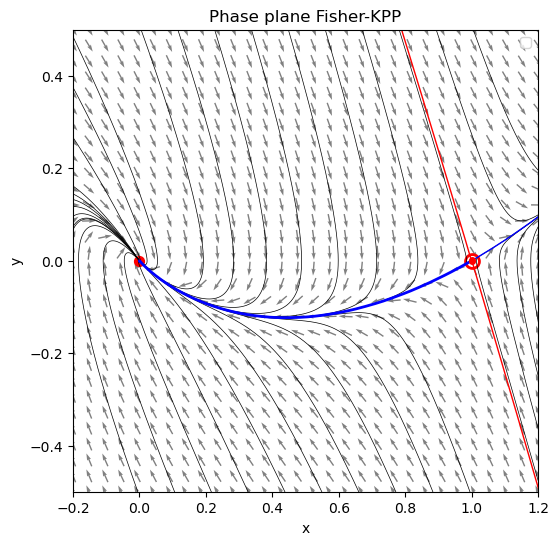
\includegraphics[scale= 0.5]{phase_fisherkpp.png}
        \end{figure}	
        \end{columns} 		
    \end{frame}

    \begin{frame}
        Approximate solution could be found by small perturbation method.

        The second order solution:
        \begin{align*}
            u_{0} &= \frac{1}{1 + e^{z/c}}\\
            u_{1} &= \frac{e^{z/c}}{\left( 1+ e^{z/c} \right)^2}\ln\left( \frac{4 e^{z/c}}{\left( 1+ e^{z/c} \right)^2} \right)\\
            u &\approx u_{0} + c^{-2} u_{1}
        \end{align*}

        \begin{figure}
            \centering
            \includegraphics[scale = 0.4]{fisher_simu.png}
        \end{figure}
    \end{frame}

    \begin{frame}{Allen-Cahn equation}
        \begin{columns}
            \column{0.5\textwidth}
            Allen-Cahn equation has reaction term which contains Allee effect.
            \begin{equation}
                \frac{\partial u}{\partial t} = \frac{\partial ^2 u} {\partial x^2} +  u (1-u) (u-a)
            \end{equation}
            The reaction term $f(u) = u(1-u)(u-a)$ ($0<a<1$) has three roots.

            \column{0.5\textwidth}
            \begin{figure}
                \centering
                \includegraphics[scale= 0.5]{allen_pu_plane.png}
            \end{figure}
        \end{columns}
    \end{frame}

    \begin{frame}
        \begin{columns}
            \column{0.4\textwidth}
            Consider the condition $a = 0.5$, we write the ODE set
        \begin{equation*}
            \begin{cases}
                \dot{u} = p\\
                \dot{p} = -cp - u(1-u)(u-a)
            \end{cases}
        \end{equation*}
            \column{0.6\textwidth}
            \begin{figure}
            \centering
            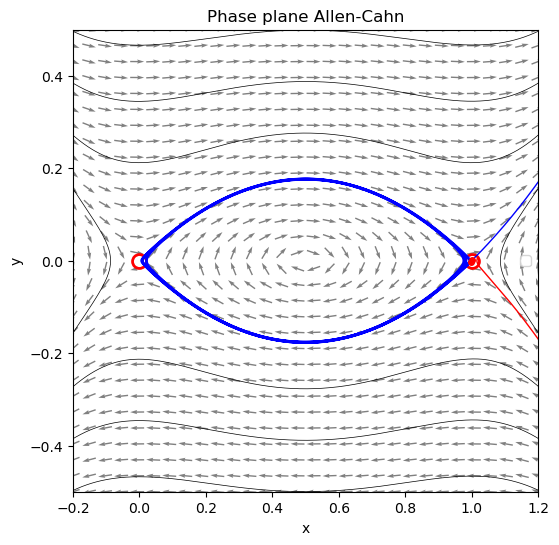
\includegraphics[scale= 0.5]{phase_allencahn.png}
        \end{figure}	
        \end{columns} 
    \end{frame}

    \begin{frame}
        When $c = 0$, the ODE could be solved.

        \begin{equation*}
            \frac{\mathrm{d}^2 u}{\mathrm{d} z^2} = u(1-u)(a-u)
        \end{equation*}
        \begin{equation*}
            u = \frac{1}{1+e^{\frac{z}{\sqrt{2}}}}
        \end{equation*}
        \begin{figure}
            \centering
            \includegraphics[scale = 0.4]{logistic.png}
        \end{figure}
    \end{frame}

    \begin{frame}
        \begin{itemize}
            \item We model spatial community dynamics using a reaction--diffusion framework with generalized Lotka--Volterra (GLV) interactions.
            
            \item Analysis of a single-species bistable system suggests that symmetric bistability can generate stable stationary interfaces.
        \end{itemize}
    \end{frame}

    \section{Coexistence as a result of dispersal}

    \subsection{Two Species Model}

    \begin{frame}{Two Species Model}
        The two-species case is the simplest example of the more general problem of multispecies coexistence. 
        \begin{equation}
            \begin{cases}
                \frac{\partial N_1}{\mathrm{d}t} = D_{1}\frac{\partial^2 N_1}{\partial x^2} + N_1 \left( r_1 - A_{1,1} N_1 - A_{1,2} N_2 \right)\\ 
                \frac{\partial N_2}{\mathrm{d}t} = D_{2}\frac{\partial^2 N_2}{\partial x^2} + N_2 \left( r_2 - A_{2,2} N_2 - A_{2,1} N_1 \right)
            \end{cases}
        \end{equation}
        The system can be nondimensionalized as
        \begin{equation}
            \begin{aligned}
                \frac{\partial u}{\partial \tau} 
                &= \frac{\partial^2 u}{\partial z^2} 
                +  u \left( 1 - u - a_{1,2} v \right),\\ 
                \frac{\partial v}{\partial \tau} 
                &= D \frac{\partial^2 v}{\partial z^2} 
                + r\, v \left( 1 - v - a_{2,1} u \right),
            \end{aligned}
        \end{equation}
    \end{frame}

    \begin{frame}{Symmetrical Condition}
        We first consider the symmetric case of the two-species system, in which $D = 1$, $r = 1$, and $a_{1,2} = a_{2,1} = a$. Under these assumptions, the system can be written in the simplified non-dimensional form,
        \begin{equation*}
            \begin{cases}
                \partial_t N_{1} = \nabla^2 N_1 + N_1(1 - N_1 - a N_2),\\
                \partial_t N_{2} = \nabla^2 N_2 + N_2(1 - N_2 - a N_1).
            \end{cases}
        \end{equation*}
    \end{frame}

    \begin{frame}
        Introduce the following linear transformation as 
        \begin{equation}
            \begin{pmatrix}
                u\\
                v
            \end{pmatrix}
            = \begin{pmatrix}
                1 & 1 \\
                1 & -1
            \end{pmatrix}
            \cdot
            \begin{pmatrix}
                N_1\\
                N_2
            \end{pmatrix},
        \end{equation}
        where the variables $u$ and $v$ represent the total population density and the population contrast between the two species.

        The system can be rewritten as 
        \begin{equation}
            \label{eqn:symme_transform}
            \begin{cases}
                \partial_t u
                = \nabla_x^2 u
                + u
                - \frac{1+a}{2}u^2
                - \frac{1-a}{2}v^2,\\
                \partial_t v
                = \nabla_x^2 v + v(1-u).
            \end{cases}
        \end{equation}
    \end{frame}

    \begin{frame}
        Approximate
        \begin{equation*}
            \partial_t u \approx 0,
            \qquad
            \nabla_x^2 u \approx 0.
        \end{equation*}

        \begin{equation}\label{eqn:u_approx_solution}
            u = \frac{1 + \sqrt{1 + (a^2-1)v^2}}{1+a}.
        \end{equation}
        Substituting it into the system for $v$ gives
        \begin{equation}
            \partial_t v
            =
            \nabla^2 v
            +
            v
            \left(
                1
                -
                \frac{1+\sqrt{1+(a^2-1)v^2}}{1+a}
            \right).
        \end{equation}
    \end{frame}

    \begin{frame}
        \begin{figure}
            \centering
            \includegraphics[scale = 0.45]{two_species_rec.png}
        \end{figure}
        This form is close to Allen-Cahn equation.
    \end{frame}

    \begin{frame}
        The effective reaction term $ f(v) = v \left( 1 - \frac{1+\sqrt{1+(a^2-1)v^2}}{1+a} \right) $
        \begin{equation*}
            f'(0)=\frac{a-1}{a+1}.
        \end{equation*}

        Consequently, the interaction front can be approximated by the Allen--Cahn traveling-wave profile (keep $v(-\infty) = -1$, $v(\infty) = 1$),
        \begin{equation}
            v(z)
            \approx
            \frac{-2}{1+e^{\sqrt{2r}\,z}} + 1,
        \end{equation}
        where
        \begin{equation}
            r=\frac{a-1}{a+1}.
        \end{equation}
    \end{frame}

    \begin{frame}
        \begin{figure}
            \centering
            \includegraphics[scale = 0.7]{symmetric_simu.pdf}
        \end{figure}
    \end{frame}

    \begin{frame}
        \begin{figure}
            \centering
            \includegraphics[scale = 0.7]{symmetric_simu_sum_diff.pdf}
        \end{figure}
    \end{frame}

    \begin{frame}
        \begin{columns}
            \column{0.5\textwidth}
            The centra slope is approximately
            \begin{equation*}
                \hat{k} = \sqrt{2r} \qquad r = \frac{a-1}{a+1} = \frac{q}{q+2}...(q = a-1)
            \end{equation*}

            \begin{equation*}
                \hat{k}|_{q\rightarrow0}\to0,
            \end{equation*}

            \begin{equation*}
                \hat{k}|_{q\to \infty}\to\sqrt{2}.
            \end{equation*}
            \column{0.5\textwidth}

            \begin{figure}[!htbp]
                \centering
                \includegraphics[scale = 0.5]{kq.png}
                {\small * Here $k$ is scaled by $\times 10$}
            \end{figure}
        \end{columns}
    \end{frame}

    \begin{frame}{Asymmetric condition}
        \begin{columns}
            \column{0.5\textwidth}
            \begin{equation*}
                \begin{aligned}
                    \partial_t N_1 &= D \nabla^2 N_1 + r N_1(1 - N_1 - 1.5 N_2)\\
                    \partial_t N_2 &= \nabla^2 N_2 + N_2(1 - N_2 - 1.5 N_1)
                \end{aligned},
            \end{equation*}
        \column{0.5\textwidth}
        \begin{figure}
            \centering
            \includegraphics[scale = 0.5]{Dr_linear.png}
            {\small \textcolor{blue}{Blue}: left, \textcolor{red}{Red}: right}
        \end{figure}
        \end{columns}
    \end{frame}

    \begin{frame}
        \begin{columns}
            \column{0.2\textwidth}
            $D=1.25$
            
            $r=0.75$
            \column{0.8\textwidth}
            \begin{figure}[!htbp]
                \centering
                \includegraphics[scale = 0.6]{insymme.pdf}
            \end{figure}
        \end{columns}
    \end{frame}

    \begin{frame}
        \begin{columns}
            \column{0.5\textwidth}
            \begin{equation*}
                \begin{aligned}
                    \partial_t N_1 &= D \, \nabla^2 N_1 + N_1(1 - N_1 - a_{1,2} N_2)\\
                    \partial_t N_2 &= \nabla^2 N_2 + N_2(1 - N_2 - 1.5 N_1)
                \end{aligned}.
            \end{equation*}
        \column{0.5\textwidth}
        \begin{figure}
            \centering
            \includegraphics[scale = 0.5]{Da_linear.png}
            {\small \textcolor{blue}{Blue}: left, \textcolor{red}{Red}: right}
        \end{figure}
        \end{columns}
    \end{frame}

    \subsection{Multi-species Model}

    \begin{frame}{Multi-species}
        \begin{equation*}
            \begin{aligned}
                \partial N_{1,i} 
                & = D_{1,i} \nabla^2 N_{1,i} 
                + r_{1,i} N_{1,i} 
                \left( 
                     1 
                     - \sum_{k} A_{ik} N_{1,k} 
                     - \sum_{\ell} A_{i\ell} N_{2,\ell} 
                \right)\\
                \partial N_{2,j} 
                &= D_{2,j}\nabla^2 N_{2,j} 
                + r_{2,j} N_{2,j} 
                \left( 
                    1 
                    - \underbrace{\sum_{\ell} A_{j\ell} N_{2,\ell}}_{intra-community} 
                    - \underbrace{\sum_{k} A_{jk} N_{1,k}}_{inter-community} 
                \right)
            \end{aligned}
        \end{equation*}
        The intra-community interaction ($A_{ik}, A_{j\ell}$) is close to self-regulation ($\approx 1$), but the inter-community interaction ($A_{i\ell}, A_{jk}$) is relatively strong.
    \end{frame}

    \begin{frame}
        \begin{equation*}
            \begin{pmatrix}
                1       &\dots&\textcolor{blue}{a}      &\textcolor{red}{b}   &\textcolor{red}{\dots}  &\textcolor{red}{b}  \\
                \dots   &\dots&\dots                    &\textcolor{red}{\dots}  &\textcolor{red}{\dots}  &\textcolor{red}{\dots}  \\
                \textcolor{blue}{a}&\dots&1             &\textcolor{red}{b}   &\textcolor{red}{\dots}  &\textcolor{red}{b}  \\
                \textcolor{red}{b}&\textcolor{red}{\dots} &\textcolor{red}{b}  &1    &\dots&\textcolor{blue}{a}  \\
                \textcolor{red}{\dots}  &\textcolor{red}{\dots}  &\textcolor{red}{\dots}                   &\dots   &\dots &\dots  \\
                \textcolor{red}{b}&\textcolor{red}{\dots} &\textcolor{red}{b}  &\textcolor{blue}{a}   &\dots&1  \\
            \end{pmatrix}
        \end{equation*}

        Because all species within the same sub-community experience identical interaction terms, the system can be reduced to the dynamics of the total sub-community biomasses, $C_n=\sum_i N_{n,i}$.
        The governing equations become
        \begin{equation*}
            \begin{aligned}
                \frac{\partial C_1}{\partial t}
                &=
                \nabla^2 C_1
                +
                C_1
                \left(
                    1
                    -
                    C_1
                    -
                    bC_2
                \right),\\
                \frac{\partial C_2}{\partial t}
                &=
                \nabla^2 C_2
                +
                C_2
                \left(
                    1
                    -
                    C_2
                    -
                    bC_1
                \right).
            \end{aligned}
        \end{equation*}
    \end{frame}

    \begin{frame}
        Spatial dynamics of a six-species community with intra-community interaction strength $a=1$, inter-community interaction strength $b=1.5$, and identical dispersal and growth rates for all species.
        \begin{figure}
            \centering
            \includegraphics[scale = 0.5]{multi_symme_simu.png}
        \end{figure}
    \end{frame}

    \begin{frame}
        Simulation of a sixteen-species community. The two subcommunities remain interactionally symmetric, with the same values of $a$ and $b$, but species are assigned different dispersal rates:
        $D=1,1.05,1.1,1.15,1.2,1.25,1.3,1.35$ for species $1$--$8$ and $9$--$16$, respectively.

        \begin{columns}
            \column{0.6\textwidth}
            \begin{figure}
                \centering
                \includegraphics[scale = 0.5]{multi_insymme_simu.png}
            \end{figure}
            \column{0.4\textwidth}
            \begin{figure}
                \centering
                \includegraphics[scale = 0.3]{multi_insymme_loss.png}
            \end{figure}
        \end{columns}
        
    \end{frame}

    \begin{frame}
        \begin{itemize}
            \item For two symmetric competing species, a stable coexistence interface emerges and is approximately logistic under weak competition.
            
            \item In asymmetric systems, stable interfaces exist under a balance between dispersal and population growth.
            
            \item Multi-species neutral communities exhibit transition fronts that follow the same qualitative dynamics as the two-species case.
        \end{itemize}
    \end{frame}

\section{$\beta$ Diversity on the Boundary}

    \begin{frame}
        \begin{figure}
            \centering
            \includegraphics[scale = 0.6]{intro/alpha_sample.png}
        \end{figure}
    \end{frame}

    \begin{frame}
        The Shannon--Weaver index is an information-theoretic measure that quantifies the uncertainty associated with randomly sampling a species. For discrete samples, the $\alpha$- and $\gamma$-diversity are defined as
        \begin{equation}
            \begin{aligned}
                \alpha_k &= -\sum_i p_{k,i} \ln(p_{k,i}), 
                \qquad p_{k,i} = \frac{N_{k,i}}{\sum_{j} N_{k,j}},\\
                \gamma &= -\sum_i q_i \ln(q_i),
                \qquad q_i = \frac{\sum_{k} N_{k,i}}{\sum_{j}\sum_{k} N_{k,j}}.
            \end{aligned}
        \end{equation}

        In addition, $\beta$-diversity measures the variation in community composition across space,
        \begin{equation}
            \beta = \frac{\gamma}{\frac{1}{n} \sum_{k} \alpha_k}.
        \end{equation}
    \end{frame}

    \begin{frame}
        \begin{figure}
            \centering
            \includegraphics[scale = 0.6]{intro/alpha_cont.png}
        \end{figure}
    \end{frame}
    
    \begin{frame}
        When continuous spatial distributions $N_i(x)$ are available (rather than discrete samples $N_{k,i}$), these definitions can be extended accordingly. The local diversity at position $x$ is defined as
        \begin{equation}
            \begin{aligned}
                \alpha(x) &= -\sum_i p_i(x) \ln\big(p_i(x)\big), 
                \qquad p_i(x) = \frac{N_i(x)}{\sum_{j} N_j(x)},\\
                \gamma &= -\sum_i q_i \ln(q_i),
                \qquad q_i = \frac{\int N_i(x)\,\mathrm{d}x}{\sum_{j} \int N_j(x)\,\mathrm{d}x}.
            \end{aligned}
        \end{equation}
        Accordingly, the continuous analogue of $\beta$-diversity is given by
        \begin{equation}\label{eqn:beta_con}
            \beta = \frac{\gamma}{\frac{1}{L} \int \alpha(x)\,\mathrm{d}x},
        \end{equation}
        where $L$ denotes the length of the spatial domain. 
    \end{frame}

    \begin{frame}{Example}
        \begin{columns}
            \column{0.6\textwidth}
            \begin{figure}
                \centering
                \includegraphics[scale = 0.45]{multi_insymme_simu.png}
            \end{figure}
            \column{0.4\textwidth}
            $\alpha$:
            \begin{figure}
                \centering
                \includegraphics[scale = 0.3]{alpha.png}
            \end{figure}
            \begin{equation*}
                \bar{\alpha}=1.654.
            \end{equation*}
            \begin{equation*}
                \gamma=2.115.
            \end{equation*}
            \begin{equation*}
                \beta
                =
                \frac{\gamma}{\bar{\alpha}}
                =
                1.279,
            \end{equation*}
        \end{columns}
    \end{frame}

    \begin{frame}
        First, a set of random sampling locations ($k = 5, 10$) was selected within the simulated spatial domain $[-1,1]$. At each sampling location $x$, the probability of observing an individual from species $i$ was assumed to be proportional to its local population abundance,
        \begin{equation*}
            p_i(x) = \frac{N_i(x)}{\sum_j N_j(x)}.
        \end{equation*}
        Then $n = 20, 50, 100$ individuals are sampled independently at each location according to the probability distribution $\{p_i(x)\}$. Consequently, the sampled abundances of the species, denoted by $n_i(x)$, followed a multinomial distribution,
        \begin{equation*}
            \mathrm{P}\left(n_1(x), n_2(x), \dots, n_S(x)\right) 
            = \frac{n!}{n_1(x)! \cdots n_S(x)!} 
            \prod_{i=1}^{S} p_i(x)^{n_i(x)},
            \qquad
            \sum_{i=1}^{S} n_i(x) = n.
        \end{equation*}
    \end{frame}

    \begin{frame}
        \begin{figure}
            \centering
            \includegraphics[scale = 0.6]{sample.png}
        \end{figure}
    \end{frame}

    \begin{frame}
        \begin{columns}
            \column{0.8\textwidth}
            \begin{figure}
                \centering
                \includegraphics[scale = 0.4]{beta_compare_MSE.png}
            \end{figure}
            \column{0.2\textwidth}
            \begin{equation*}
                \text{MSE} = \frac{1}{n}\sum (\beta - \hat{\beta})^2
            \end{equation*}
        \end{columns}
    \end{frame}

    \begin{frame}
        \begin{table}
        \centering
        \begin{tabular}{cccccc}
        \toprule
        $n_{\text{points}}$ & $k$ & MSE (Discrete) & MSE (Continuous) & $p$-value (t-test) & $p$-value (Levene) \\
        \midrule
        5  & 20  & 0.018911 & 0.010848 & $2.43\times10^{-12}$ & 0.626610 \\
        5  & 50  & 0.007675 & 0.011208 & $2.25\times10^{-6}$  & 0.537370 \\
        5  & 100 & 0.006730 & 0.009625 & $4.89\times10^{-5}$  & 0.761784 \\
        10 & 20  & 0.031366 & 0.006810 & $2.07\times10^{-15}$ & 0.240839 \\
        10 & 50  & 0.007628 & 0.002553 & $3.55\times10^{-11}$ & 0.025949 \\
        10 & 100 & 0.004579 & 0.002610 & $5.35\times10^{-5}$  & 0.096430 \\
        \bottomrule
        \end{tabular}
        \end{table}
    \end{frame}

    \begin{frame}
        \begin{itemize}
            \item Larger sample sizes lead to more accurate estimates of $\beta$-diversity.
            
            \item Continuous-distribution fitting is generally better than direct discrete estimation.
            
            \item The advantage of the continuous approach becomes more apparent as the number of sampling locations increases.
        \end{itemize}
    \end{frame}

\section{Discussion}

    \begin{frame}{Why can a logistic function provide a good approximation?}

    For species $i$ belonging to community $1$ (the left community), the reaction--diffusion dynamics are

    \begin{equation*}
        \partial_t N_{1,i}
        =
        D_{1,i}\nabla^2 N_{1,i}
        +
        r_{1,i}N_{1,i}
        \left(
            1
            -
            \sum_k A_{ik}N_{1,k}
            -
            \sum_\ell A_{i\ell}N_{2,\ell}
        \right).
    \end{equation*}

    Far inside the region dominated by community $1$, the abundance of species from community $2$ approaches zero, i.e.,
    $N_{2,\ell}\rightarrow 0$, while the abundances of species in community $1$ approach their equilibrium values
    ${N}_{1,k}^*$.
    In this limit, the system is approximately equivalent to the local dynamics of community $1$ linearized around its stable equilibrium.

    \end{frame}

    \begin{frame}
        Let $\mathbf{N^*}_1$ denote the equilibrium state of community $1$. Linear stability analysis gives

        \begin{equation*}
            \partial_t \delta \mathbf N
            =
            D\nabla^2 \delta \mathbf N
            +
            J(\mathbf{N^*}_1)\delta \mathbf N,
        \end{equation*}

        where $J(\mathbf{N^*}_1)$ is the Jacobian matrix evaluated at the equilibrium.
        If the dominant eigenvalues of $J$ are real and negative, perturbations decay exponentially with distance from the equilibrium state. 
    \end{frame}

    \begin{frame}
        Consequently, for sufficiently large $|x|$,
        \begin{equation*}
            N_{1,i}(x)- N_{1,i}^*
            \propto
            e^{-c_i |x|},
        \end{equation*}
        for some positive constant $c_i$.
        A similar argument applies on the opposite side of the interface. In the region dominated by community $2$, the abundance of species $i$ from community $1$ approaches zero exponentially,
        \begin{equation*}
            N_{1,i}(x)
            \propto
            e^{-d_i |x|},
        \end{equation*}
        with $d_i>0$.
    \end{frame}

    \begin{frame}
        \begin{figure}
            \centering
            \includegraphics[scale = 0.6]{transition_showcase.png}
        \end{figure}
    \end{frame}

    \iffalse
    \begin{frame}
        Therefore, regardless of the detailed dynamics within the transition zone, the abundance profile of each species is expected to connect two asymptotic states through exponential convergence on both sides of the interface. The logistic function naturally possesses exactly this property: it exhibits a rapid transition near its center while approaching its limiting values exponentially in both tails. This provides a theoretical explanation for why logistic curves offer an excellent approximation to the equilibrium species distributions observed in our simulations.
    \end{frame}
    \fi

    \begin{frame}{Limited Dispersal}
        \begin{equation*}
            \partial_t u
            =
            \nabla\left(
                D(u)\nabla u
            \right),
            \qquad
            D(u)
            =
            \frac{u^b}{(1-u)^b}.
        \end{equation*}

        \begin{figure}
            \centering
            \includegraphics[scale = 0.6]{nonliear.pdf}
        \end{figure}
    \end{frame}

    \begin{frame}{Pattern}
        \begin{columns}
            \column{0.4\textwidth}
            \begin{figure}
                \centering
                \includegraphics[scale = 0.3]{pattern_1D.png}
            \end{figure}
            \column{0.6\textwidth}
            \begin{figure}
                \centering
                \includegraphics[scale = 0.4]{2D_pattern.pdf}
            \end{figure}
        \end{columns}
    \end{frame}

    \maketitle

\end{document}